\documentclass{tufte-handout}

\title{Discrete Probabilistic Programming Languages\thanks{CS7470 Fall 2023: Foundations of Probabilistic Programming.}}


\newcommand{\varset}[0]{\mathcal{V}}

\author[]{Steven Holtzen\\s.holtzen@northeastern.edu}

%\date{28 March 2010} % without \date command, current date is supplied

%\geometry{showframe} % display margins for debugging page layout
\setcounter{secnumdepth}{1}

\usepackage{graphicx} % allow embedded images
  \setkeys{Gin}{width=\linewidth,totalheight=\textheight,keepaspectratio}
  \graphicspath{{graphics/}} % set of paths to search for images
\usepackage{amsmath,amssymb,amsthm}  % extended mathematics
\usepackage{booktabs} % book-quality tables
\usepackage{units}    % non-stacked fractions and better unit spacing
\usepackage{multicol} % multiple column layout facilities
\usepackage{lipsum}   % filler text
\usepackage{fancyvrb} % extended verbatim environments
  \fvset{fontsize=\normalsize}% default font size for fancy-verbatim environments
\usepackage{listings}
\usepackage{tikz}
\usepackage{mathpartir}
\usepackage{subcaption}
\usepackage{mdframed}
\usepackage{epigraph}
\usepackage{enumitem}
\usepackage{stmaryrd}

\usetikzlibrary{shapes.geometric}


\usepackage[ruled,linesnumbered]{algorithm2e}
\SetKwComment{Comment}{/* }{ */}
\newcommand{\indep}{\perp \!\!\! \perp}

\tikzset{
  treenode/.style = {shape=rectangle, rounded corners,
                     draw, align=center,
                     },
  root/.style     = {treenode, font=\Large, bottom color=red!30},
  env/.style      = {treenode, font=\ttfamily\normalsize},
  dummy/.style    = {circle,draw}
}

% tikz
\usetikzlibrary{patterns,calc,backgrounds}


% TIKZ
\tikzstyle{nnf}=[
  >=stealth,font=\small,auto,scale=0.7,every node/.style={scale=0.7}
]
\tikzstyle{extnode}=[
  draw,circle,inner sep=2pt,fill=white
]

\tikzstyle{leafnode}=[
  draw,fill=gray!20,inner sep=3.5pt
]
\tikzstyle{constnode}=[
  draw,fill=white,inner sep=3.5pt
]
\tikzstyle{label}=[
  fill=white,inner sep=2.5pt
]

\tikzstyle{acarrow}=[
    decoration={markings,mark=at position 1 with {\arrow[scale=0.6]{>}}},
    postaction={decorate},
    shorten >=0.4pt,
    >=latex,
    line width=0.1
]

\tikzstyle{bnarrow}=[
    decoration={markings,mark=at position 1 with {\arrow[scale=1.5]{>}}},
    postaction={decorate},
    shorten >=0.7pt,
    >=latex,
    line width=0.3
]
\tikzstyle{bayesnet}=[
  >=latex, thick, auto
]
\tikzstyle{bnnode}=[
  draw,ellipse,minimum size=7mm,inner sep=1pt,font=\small
]
\tikzstyle{cpt}=[
  font=\footnotesize
]

\tikzstyle{graph}=[
  >=stealth,font=\small,auto,scale=1,every node/.style={scale=1}
]
\tikzstyle{node}=[
  draw,circle,inner sep=3pt,fill=white
]

% BDDs

\tikzstyle{bdd}=[
  >=latex, thick, >=stealth, font=\small,auto,scale=0.9,every node/.style={scale=0.9}
]
\tikzstyle{bddnode}=[
  draw,circle,inner sep=0pt,fill=white,minimum size=5.5mm
]

\tikzstyle{bddtriangle}=[
  draw, regular polygon, regular polygon sides = 3,inner sep=1pt,fill=white,minimum size=5.5mm
]

\tikzstyle{highedge}=[
    line width=0.9
]
\tikzstyle{lowedge}=[
    line width=0.9,dotted
]
\tikzstyle{bddterminal}=[
  draw,fill=gray!20,inner sep=2.5pt, font=\small
]

\lstdefinestyle{compact}{
  \ttfamily\tiny
}


\usetikzlibrary{positioning}

\newtheorem{theorem}{Theorem}
\newtheorem{definition}{Definition}
\newtheorem{conjecture}{Conjecture}
\newtheorem{lemma}{Lemma}
\newtheorem{exercise}{Exercise}
\newtheorem{remark}{Remark}


\usepackage{xcolor}

\definecolor{codegreen}{rgb}{0,0.6,0}
\definecolor{codegray}{rgb}{0.5,0.5,0.5}
\definecolor{codepurple}{rgb}{0.58,0,0.82}
\definecolor{backcolour}{rgb}{0.95,0.95,0.92}

\lstdefinestyle{mystyle}{
    backgroundcolor=\color{backcolour},   
    commentstyle=\color{codegreen},
    keywordstyle=\color{magenta},
    numberstyle=\tiny\color{codegray},
    stringstyle=\color{codepurple},
    basicstyle=\ttfamily\footnotesize,
    breakatwhitespace=false,         
    breaklines=true,                 
    captionpos=b,                    
    keepspaces=true,                 
    numbers=left,                    
    numbersep=5pt,                  
    showspaces=false,                
    showstringspaces=false,
    showtabs=false,                  
    tabsize=2
}

\lstset{style=mystyle}

\newcommand{\defn}[1]{\textbf{#1}}
\newcommand{\dbracket}[1]{\left \llbracket {#1} \right \rrbracket}
\newcommand{\dist}[1]{\mathtt{Dist}(#1)}
\newcommand{\true}[0]{\texttt{true}}
\newcommand{\te}[0]{\texttt{e}}
\newcommand{\false}[0]{\texttt{false}}
\newcommand{\real}[0]{\mathbb{R}}
\newcommand{\rational}[0]{\mathbb{Q}}
\newcommand{\lebesgue}[0]{\mathbb{L}}
\newcommand{\eval}[0]{\mathrm{ev}}
\newcommand{\disc}[0]{\textsc{Disc}}
\newcommand{\borel}[0]{\mathcal{B}}
\newcommand{\ent}[0]{\mathbb{S}}
\newcommand{\prog}[0]{\texttt{p}}
\newcommand{\bool}[0]{\mathbb{B}}
\newcommand{\cont}[0]{\textsc{Cont}}
\newcommand{\prop}[0]{\textsc{Prop}}
\newcommand{\bdd}[0]{\textsc{Bdd}}
\newcommand{\robdd}[0]{\textsc{Robdd}}
\newcommand{\compiles}[0]{\rightsquigarrow}

\newcommand{\bddtriangle}[1]{
    \begin{tikzpicture}
    \node [bddtriangle] {#1};
    \end{tikzpicture}}
\newcommand{\bddtrue}[0]{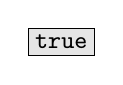
\begin{tikzpicture}
      \node [bddterminal] {$\true$};
    \end{tikzpicture}}
\newcommand{\bddfalse}[0]{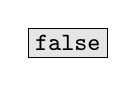
\begin{tikzpicture}
      \node [bddterminal] {$\false$};
    \end{tikzpicture}}


% Standardize command font styles and environments
\newcommand{\doccmd}[1]{\texttt{\textbackslash#1}}% command name -- adds backslash automatically
\newcommand{\docopt}[1]{\ensuremath{\langle}\textrm{\textit{#1}}\ensuremath{\rangle}}% optional command argument
\newcommand{\docarg}[1]{\textrm{\textit{#1}}}% (required) command argument
\newcommand{\docenv}[1]{\textsf{#1}}% environment name
\newcommand{\docpkg}[1]{\texttt{#1}}% package name
\newcommand{\doccls}[1]{\texttt{#1}}% document class name
\newcommand{\docclsopt}[1]{\texttt{#1}}% document class option name
\newenvironment{docspec}{\begin{quote}\noindent}{\end{quote}}% command specification environment



\begin{document}
\maketitle% this prints the handout title, author, and date

\begin{itemize}
  \item Goal for today: compile a simple discrete PPL to BDD
\end{itemize}

\section{Compositional compilation of BDDs}
\begin{itemize}
  \item So far we have compiled by inducting on variables
  \item \textbf{Problem}: this is not \emph{compositional}! A compilation
  process is compositional if it works by compiling big programs out of 
  smaller sub-programs. I.e., it would have a rule that looks something like:
  \begin{mathpar}
    \inferrule{\alpha \compiles \alpha' \and \beta \compiles \beta'}{
      \alpha \land \beta \compiles \alpha' \times \beta'
    }
  \end{mathpar}
  \item Compositional compilation is great: gives us modular reasoning 
  about performance, ... (other reasons?)
  \item \textbf{Goal}: Design a compositional process for compiling \prop$_S$ to 
  \bdd{}

  \item How can we build big BDDs out of smaller ones? Define a way to compose together 
  BDDs, again using a type-directed step-relation $\Gamma \vdash \alpha_1 \land
  \alpha_2 \Downarrow \beta$, shown in Figure~\ref{fig:bdd}.

  
  \begin{theorem}[Correctness]
    If $\Gamma \vdash \alpha_1$, $\Gamma \vdash \alpha_2$, and $\Gamma \vdash \alpha_1 \land \alpha_2 \Downarrow \beta$, 
    then $\dbracket{\alpha_1} \cap \dbracket{\alpha_2} = \dbracket{\beta}$.
  \end{theorem}
  \begin{proof}
    By simultaneous structural induction on syntax of BDDs (note that we need to
    perform simultaneous induction since there are two BDDs at play here). The
    rules in Figure~\ref{fig:bdd} are exhaustive (i.e., every pair of syntactic BDDs matches
    exactly one of these structural rules), so we can proceed by case analysis on each
    of the compilation rules. The base cases are quite simple and we elide them here. The
    interesting cases are the inductive cases.

    We will show the case for \textsc{(SameVarNE)}.  Assume that $\Gamma \vdash \alpha_1 \land
    \alpha_3 \Downarrow \alpha_{13}$ and $\Gamma \vdash \alpha_2 \land \alpha_4 \Downarrow
    \alpha_{24}$. As usual, our inductive hypothesis assumes that the theorem 
    holds for compiled subterms:
    \begin{itemize}
      \item $\dbracket{\Gamma \vdash \alpha_1} \cap \dbracket{\Gamma \vdash \alpha_3} = \dbracket{\Gamma \vdash \alpha_{13}}$
      \item $\dbracket{\Gamma \vdash \alpha_2} \cap \dbracket{\Gamma \vdash \alpha_4} = \dbracket{\Gamma \vdash \alpha_{24}}$
    \end{itemize}

    We want to show that:

    \begin{align*}
    \dbracket{x :: \Gamma \vdash 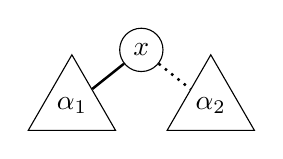
\begin{tikzpicture}
      \node (x) [bddnode] {$x$};
      \node (a1) at ($(x) + (-25bp, -20pt)$) [bddtriangle] {$\alpha_1$};
      \node (a2) at ($(x) + (25bp, -20pt)$) [bddtriangle] {$\alpha_2$};
    \begin{scope}[on background layer]
      \draw [highedge] (x) -- (a1);
      \draw [lowedge] (x) -- (a2);
    \end{scope}
    \end{tikzpicture}}
    \bigcap
    \dbracket{x :: \Gamma \vdash
    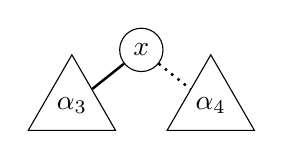
\begin{tikzpicture}
      \node (x) [bddnode] {$x$};
      \node (a1) at ($(x) + (-25bp, -20pt)$) [bddtriangle] {$\alpha_3$};
      \node (a2) at ($(x) + (25bp, -20pt)$) [bddtriangle] {$\alpha_4$};
    \begin{scope}[on background layer]
      \draw [highedge] (x) -- (a1);
      \draw [lowedge] (x) -- (a2);
    \end{scope}
    \end{tikzpicture}
    } =
    \dbracket{x :: \Gamma \vdash 
    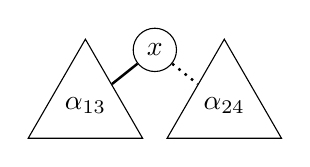
\begin{tikzpicture}
      \node (x) [bddnode] {$x$};
      \node (a1) at ($(x) + (-25bp, -20pt)$) [bddtriangle] {$\alpha_{13}$};
      \node (a2) at ($(x) + (25bp, -20pt)$) [bddtriangle] {$\alpha_{24}$};
    \begin{scope}[on background layer]
      \draw [highedge] (x) -- (a1);
      \draw [lowedge] (x) -- (a2);
    \end{scope}
    \end{tikzpicture}
    }
  \end{align*}

  We reason forward:
  {\footnotesize 
  \begin{align*}
    \dbracket{x :: \Gamma \vdash 
    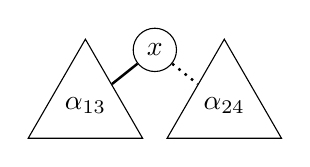
\begin{tikzpicture}
      \node (x) [bddnode] {$x$};
      \node (a1) at ($(x) + (-25bp, -20pt)$) [bddtriangle] {$\alpha_{13}$};
      \node (a2) at ($(x) + (25bp, -20pt)$) [bddtriangle] {$\alpha_{24}$};
    \begin{scope}[on background layer]
      \draw [highedge] (x) -- (a1);
      \draw [lowedge] (x) -- (a2);
    \end{scope}
    \end{tikzpicture}
    } &=
    [x \mapsto \true] \otimes \dbracket{\Gamma \vdash \alpha_{13}} ~\bigcup~ [x \mapsto \false] \otimes \dbracket{\Gamma \vdash \alpha_{24}} \\
    &= [x \mapsto \true] \otimes \Big( \dbracket{\Gamma \vdash \alpha_1} \cap \dbracket{\Gamma \vdash \alpha_3} \Big)
      ~\bigcup~ [x \mapsto \false] \otimes \Big( \dbracket{\Gamma \vdash \alpha_2} \cap \dbracket{\Gamma \vdash \alpha_4} \Big)
      & \text{By I.H.} \\
    &= \Big( [x \mapsto \true] \dbracket{\Gamma \vdash \alpha_1} \cap [x \mapsto \true] \dbracket{\Gamma \vdash \alpha_3} \Big)
      ~\bigcup~  \Big([x \mapsto \false] \dbracket{\Gamma \vdash \alpha_2} \cap [x \mapsto \false]\dbracket{\Gamma \vdash \alpha_4} \Big)
      & (\star)\\
    &= \Big( [x \mapsto \true] \dbracket{\Gamma \vdash \alpha_1} \cup [x \mapsto \false] \dbracket{\Gamma \vdash \alpha_2} \Big)
      ~\bigcap~  \Big([x \mapsto \true] \dbracket{\Gamma \vdash \alpha_1} \cup [x \mapsto \false]\dbracket{\Gamma \vdash \alpha_4} \Big)
      & (\dagger) \\ 
    &=     \dbracket{x :: \Gamma \vdash 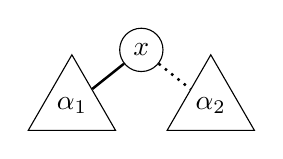
\begin{tikzpicture}
      \node (x) [bddnode] {$x$};
      \node (a1) at ($(x) + (-25bp, -20pt)$) [bddtriangle] {$\alpha_1$};
      \node (a2) at ($(x) + (25bp, -20pt)$) [bddtriangle] {$\alpha_2$};
    \begin{scope}[on background layer]
      \draw [highedge] (x) -- (a1);
      \draw [lowedge] (x) -- (a2);
    \end{scope}
    \end{tikzpicture}}
    \bigcap
    \dbracket{x :: \Gamma \vdash
    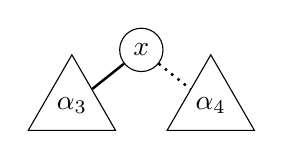
\begin{tikzpicture}
      \node (x) [bddnode] {$x$};
      \node (a1) at ($(x) + (-25bp, -20pt)$) [bddtriangle] {$\alpha_3$};
      \node (a2) at ($(x) + (25bp, -20pt)$) [bddtriangle] {$\alpha_4$};
    \begin{scope}[on background layer]
      \draw [highedge] (x) -- (a1);
      \draw [lowedge] (x) -- (a2);
    \end{scope}
    \end{tikzpicture}
    }
  \end{align*}
  }

  where $(\star)$ follows from a simple lemma that $\otimes$ distributes over intersection 
  and $(\dagger)$ follows from distributivity properties of union and intersection, 
  in particular the fact that for any sets $A,B,C,D$ it is the case that $(A \cup B) \cap (C \cup D) = 
  (A \cap C) \cup (B \cap D)$.\sidenote{This set theory property has a nice
  ``proof by Venn-diagram''; draw the Venn-diagram of these sets to see this
  fact clearly.}
  
  \end{proof}

  \item We would also like to ensure that our compilation rules produce reduced and ordered 
  BDDs. We can formalize this with a type-preservation theorem:
  \begin{theorem}[Type preservation]
    If $\Gamma \vdash \alpha_1$, $\Gamma \vdash \alpha_2$, and $\Gamma \vdash \alpha_1 \land \alpha_2 \Downarrow \alpha$, 
    then $\Gamma \vdash \alpha$.
  \end{theorem}

  \item These rules are called \emph{bottom-up BDD compilation}~\citep{darwiche2002knowledge,oztok2015top}. 
  \item There are several other compositional BDD operations we won't have time
  to explain in lecture, but you can use in your lab, like disjunction, negation, substitution, 
  and existential quantification.
  \item Why might one prefer one mode of compilation over the other? Do they
  have different runtime cost? \emph{Yes!}
  \item \textbf{Exercise}: Give example families of formulae where
  top-down compilation is faster than bottom-up and vice-versa.
\end{itemize}

  \begin{figure}
  \begin{mathpar}
    \inferrule{}{\Gamma \vdash \bddtrue{} \land \alpha \Downarrow \alpha} \and 
    \inferrule{}{\Gamma \vdash \alpha \land \bddtrue{} \Downarrow \alpha} \\
    \inferrule{}{\Gamma \vdash \bddfalse{} \land \alpha \Downarrow \bddfalse{}} \and 
    \inferrule{}{\Gamma \vdash \alpha \land \bddfalse{} \Downarrow \bddfalse{}} \\

    \inferrule*[Right={\textsc{(SameVarNE)}}]{\Gamma \vdash \alpha_1 \land \alpha_3 \compiles \alpha_{13} \and 
    \Gamma \vdash \alpha_2 \land \alpha_4 \compiles \alpha_{24} \and 
    \alpha_{13} \ne \alpha_{24}
    }{x :: \Gamma \vdash 
    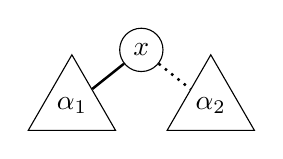
\begin{tikzpicture}
      \node (x) [bddnode] {$x$};
      \node (a1) at ($(x) + (-25bp, -20pt)$) [bddtriangle] {$\alpha_1$};
      \node (a2) at ($(x) + (25bp, -20pt)$) [bddtriangle] {$\alpha_2$};
    \begin{scope}[on background layer]
      \draw [highedge] (x) -- (a1);
      \draw [lowedge] (x) -- (a2);
    \end{scope}
    \end{tikzpicture}
    \land
    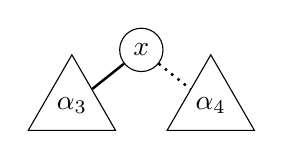
\begin{tikzpicture}
      \node (x) [bddnode] {$x$};
      \node (a1) at ($(x) + (-25bp, -20pt)$) [bddtriangle] {$\alpha_3$};
      \node (a2) at ($(x) + (25bp, -20pt)$) [bddtriangle] {$\alpha_4$};
    \begin{scope}[on background layer]
      \draw [highedge] (x) -- (a1);
      \draw [lowedge] (x) -- (a2);
    \end{scope}
    \end{tikzpicture}
    \Downarrow 
    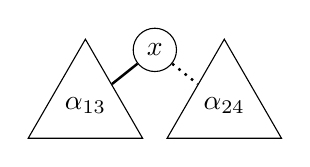
\begin{tikzpicture}
      \node (x) [bddnode] {$x$};
      \node (a1) at ($(x) + (-25bp, -20pt)$) [bddtriangle] {$\alpha_{13}$};
      \node (a2) at ($(x) + (25bp, -20pt)$) [bddtriangle] {$\alpha_{24}$};
    \begin{scope}[on background layer]
      \draw [highedge] (x) -- (a1);
      \draw [lowedge] (x) -- (a2);
    \end{scope}
    \end{tikzpicture}
    }

    \\

    \inferrule*[Right={\textsc{(SameVarEQ)}}]{\Gamma \vdash \alpha_1 \land \alpha_3 \compiles \alpha_{13} \and 
    \Gamma \vdash \alpha_2 \land \alpha_4 \compiles \alpha_{24} \and 
    \alpha_{13} = \alpha_{24}
    }{x :: \Gamma \vdash 
    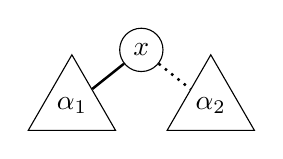
\begin{tikzpicture}
      \node (x) [bddnode] {$x$};
      \node (a1) at ($(x) + (-25bp, -20pt)$) [bddtriangle] {$\alpha_1$};
      \node (a2) at ($(x) + (25bp, -20pt)$) [bddtriangle] {$\alpha_2$};
    \begin{scope}[on background layer]
      \draw [highedge] (x) -- (a1);
      \draw [lowedge] (x) -- (a2);
    \end{scope}
    \end{tikzpicture}
    \land
    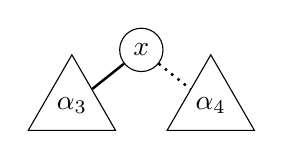
\begin{tikzpicture}
      \node (x) [bddnode] {$x$};
      \node (a1) at ($(x) + (-25bp, -20pt)$) [bddtriangle] {$\alpha_3$};
      \node (a2) at ($(x) + (25bp, -20pt)$) [bddtriangle] {$\alpha_4$};
    \begin{scope}[on background layer]
      \draw [highedge] (x) -- (a1);
      \draw [lowedge] (x) -- (a2);
    \end{scope}
    \end{tikzpicture}
    \Downarrow 
    \bddtriangle{$\alpha_{24}$}
    } 

    \\

    \inferrule*[Right=\textsc{(Weaken)}]{x \ne y \ne z \and 
    \Gamma \vdash 
    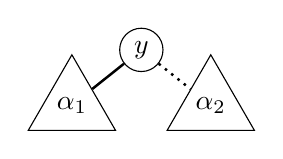
\begin{tikzpicture}
      \node (x) [bddnode] {$y$};
      \node (a1) at ($(x) + (-25bp, -20pt)$) [bddtriangle] {$\alpha_1$};
      \node (a2) at ($(x) + (25bp, -20pt)$) [bddtriangle] {$\alpha_2$};
    \begin{scope}[on background layer]
      \draw [highedge] (x) -- (a1);
      \draw [lowedge] (x) -- (a2);
    \end{scope}
    \end{tikzpicture}
    \land
    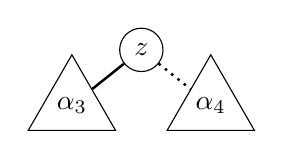
\begin{tikzpicture}
      \node (x) [bddnode] {$z$};
      \node (a1) at ($(x) + (-25bp, -20pt)$) [bddtriangle] {$\alpha_3$};
      \node (a2) at ($(x) + (25bp, -20pt)$) [bddtriangle] {$\alpha_4$};
    \begin{scope}[on background layer]
      \draw [highedge] (x) -- (a1);
      \draw [lowedge] (x) -- (a2);
    \end{scope}
    \end{tikzpicture}
    \Downarrow 
    \bddtriangle{$\alpha$}
    }{x :: \Gamma \vdash 
    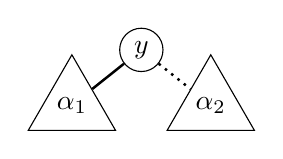
\begin{tikzpicture}
      \node (x) [bddnode] {$y$};
      \node (a1) at ($(x) + (-25bp, -20pt)$) [bddtriangle] {$\alpha_1$};
      \node (a2) at ($(x) + (25bp, -20pt)$) [bddtriangle] {$\alpha_2$};
    \begin{scope}[on background layer]
      \draw [highedge] (x) -- (a1);
      \draw [lowedge] (x) -- (a2);
    \end{scope}
    \end{tikzpicture}
    \land
    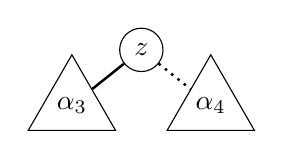
\begin{tikzpicture}
      \node (x) [bddnode] {$z$};
      \node (a1) at ($(x) + (-25bp, -20pt)$) [bddtriangle] {$\alpha_3$};
      \node (a2) at ($(x) + (25bp, -20pt)$) [bddtriangle] {$\alpha_4$};
    \begin{scope}[on background layer]
      \draw [highedge] (x) -- (a1);
      \draw [lowedge] (x) -- (a2);
    \end{scope}
    \end{tikzpicture}
    \Downarrow 
    \bddtriangle{$\alpha$}
    }

    \\

    \inferrule*[Right=\textsc{(ParNE)}]{x \ne y \and 
    \Gamma \vdash 
    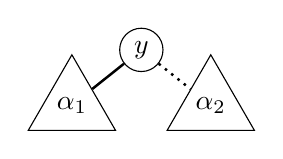
\begin{tikzpicture}
      \node (x) [bddnode] {$y$};
      \node (a1) at ($(x) + (-25bp, -20pt)$) [bddtriangle] {$\alpha_1$};
      \node (a2) at ($(x) + (25bp, -20pt)$) [bddtriangle] {$\alpha_2$};
    \begin{scope}[on background layer]
      \draw [highedge] (x) -- (a1);
      \draw [lowedge] (x) -- (a2);
    \end{scope}
    \end{tikzpicture}
    \land
    \bddtriangle{$\alpha_1$}
    \Downarrow 
    \alpha_{y_1}
    \and 
    \Gamma \vdash 
    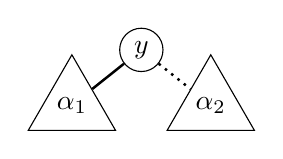
\begin{tikzpicture}
      \node (x) [bddnode] {$y$};
      \node (a1) at ($(x) + (-25bp, -20pt)$) [bddtriangle] {$\alpha_1$};
      \node (a2) at ($(x) + (25bp, -20pt)$) [bddtriangle] {$\alpha_2$};
    \begin{scope}[on background layer]
      \draw [highedge] (x) -- (a1);
      \draw [lowedge] (x) -- (a2);
    \end{scope}
    \end{tikzpicture}
    \land
    \bddtriangle{$\alpha_2$}
    \Downarrow 
    \alpha_{y_2}
    \and 
    \alpha_{y_1} \ne \alpha_{y_2}
    }{x :: \Gamma \vdash 
    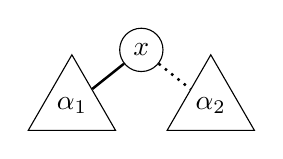
\begin{tikzpicture}
      \node (x) [bddnode] {$x$};
      \node (a1) at ($(x) + (-25bp, -20pt)$) [bddtriangle] {$\alpha_1$};
      \node (a2) at ($(x) + (25bp, -20pt)$) [bddtriangle] {$\alpha_2$};
    \begin{scope}[on background layer]
      \draw [highedge] (x) -- (a1);
      \draw [lowedge] (x) -- (a2);
    \end{scope}
    \end{tikzpicture}
    \land
    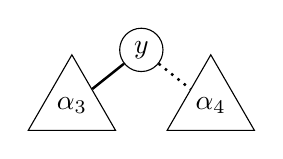
\begin{tikzpicture}
      \node (x) [bddnode] {$y$};
      \node (a1) at ($(x) + (-25bp, -20pt)$) [bddtriangle] {$\alpha_3$};
      \node (a2) at ($(x) + (25bp, -20pt)$) [bddtriangle] {$\alpha_4$};
    \begin{scope}[on background layer]
      \draw [highedge] (x) -- (a1);
      \draw [lowedge] (x) -- (a2);
    \end{scope}
    \end{tikzpicture}
    \Downarrow 
    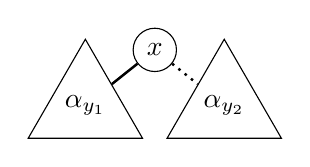
\begin{tikzpicture}
      \node (x) [bddnode] {$x$};
      \node (a1) at ($(x) + (-25bp, -20pt)$) [bddtriangle] {$\alpha_{y_1}$};
      \node (a2) at ($(x) + (25bp, -20pt)$) [bddtriangle] {$\alpha_{y_2}$};
    \begin{scope}[on background layer]
      \draw [highedge] (x) -- (a1);
      \draw [lowedge] (x) -- (a2);
    \end{scope}
    \end{tikzpicture}
    }

    \\

    \inferrule*[Right=\textsc{(ParEQ)}]{x \ne y \and 
    \Gamma \vdash 
    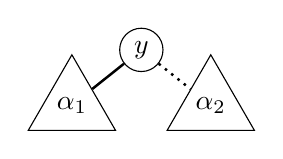
\begin{tikzpicture}
      \node (x) [bddnode] {$y$};
      \node (a1) at ($(x) + (-25bp, -20pt)$) [bddtriangle] {$\alpha_1$};
      \node (a2) at ($(x) + (25bp, -20pt)$) [bddtriangle] {$\alpha_2$};
    \begin{scope}[on background layer]
      \draw [highedge] (x) -- (a1);
      \draw [lowedge] (x) -- (a2);
    \end{scope}
    \end{tikzpicture}
    \land
    \bddtriangle{$\alpha_1$}
    \Downarrow 
    \alpha_{y_1}
    \and 
    \Gamma \vdash 
    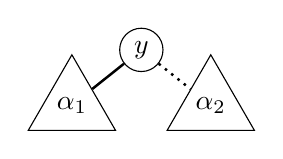
\begin{tikzpicture}
      \node (x) [bddnode] {$y$};
      \node (a1) at ($(x) + (-25bp, -20pt)$) [bddtriangle] {$\alpha_1$};
      \node (a2) at ($(x) + (25bp, -20pt)$) [bddtriangle] {$\alpha_2$};
    \begin{scope}[on background layer]
      \draw [highedge] (x) -- (a1);
      \draw [lowedge] (x) -- (a2);
    \end{scope}
    \end{tikzpicture}
    \land
    \bddtriangle{$\alpha_2$}
    \Downarrow 
    \alpha_{y_2}
    \and 
    \alpha_{y_1} = \alpha_{y_2}
    }{x :: \Gamma \vdash 
    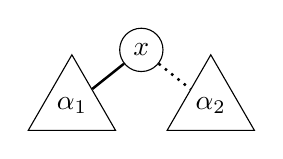
\begin{tikzpicture}
      \node (x) [bddnode] {$x$};
      \node (a1) at ($(x) + (-25bp, -20pt)$) [bddtriangle] {$\alpha_1$};
      \node (a2) at ($(x) + (25bp, -20pt)$) [bddtriangle] {$\alpha_2$};
    \begin{scope}[on background layer]
      \draw [highedge] (x) -- (a1);
      \draw [lowedge] (x) -- (a2);
    \end{scope}
    \end{tikzpicture}
    \land
    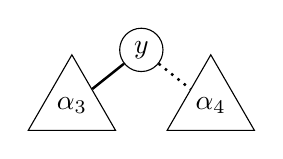
\begin{tikzpicture}
      \node (x) [bddnode] {$y$};
      \node (a1) at ($(x) + (-25bp, -20pt)$) [bddtriangle] {$\alpha_3$};
      \node (a2) at ($(x) + (25bp, -20pt)$) [bddtriangle] {$\alpha_4$};
    \begin{scope}[on background layer]
      \draw [highedge] (x) -- (a1);
      \draw [lowedge] (x) -- (a2);
    \end{scope}
    \end{tikzpicture}
    \Downarrow 
    \alpha_{y_2}
    }
  \end{mathpar}
  \caption{Rules for compiling BDDs.}
  \label{fig:bdd}
\end{figure}

\bibliographystyle{plainnat}
\bibliography{../bib}


\end{document}